
\chapter{Détection des anomalies de la route}

Avec cette évolution dans le domaine des mobiles, il est possible de développer un système pratique et efficace à faible coût et
 recueilli divers types d'informations afin de détecter la qualité de la surface des routes et aussi les anomalies routières telles
  que les ralentisseurs et les nids de-poule.

\section{Travaux Connexes}

\subsection{Wolverine}
Wolverine est \cite{bhoraskarWolverineTrafficRoad2012}une méthode non intrusive qui utilise  des données de capteurs des smartphones pour déterminer les conditions et l'état de la route, et utilise aussi des techniques d'apprentissage automatique “Machine learning” (clustering K-means et Support Vector Machine (SVM)) afin de la surveillance et suivi de l'état de la route
le chemin de ce travail consiste a deux étape: un algorithme pour réorienter virtuellement les axes de coordonnées d'un téléphone désorienté  et techniques d'apprentissage automatique pour identifier les événements de bosse et de freinage.\newline
Pour la 1ere étape ils ont développé une application qui traite les lectures de l'accéléromètre et du magnétomètre ainsi que les informations GPS et produit l'accélération linéaire du mobile, dans le cadre de référence du véhicule, ils ont développé un algorithme qui etude les axe x,y,z du téléphone et étude aussi les axes x’ y’ z’ de la véhicule.\newline
 La 2ème étape consistera à utiliser un algorithme d'apprentissage non supervisé de clustering K-means, avec K = 2, pour partitionner l'ensemble des points de données en deux classes; Ces classes sont ensuite étiquetées manuellement comme bosselées ou lisses (Bumby; smoothy)\newline
Une fois cet étiquetage manuel terminé, ils auront  un ensemble de points de données étiquetés. Ceux-ci sont ensuite utilisés pour former un classificateur Support Vector Machine. Ce SVM entraîné, à son tour, est utilisé pour classer les points de données qui sont générés pendant la phase de test, et donc pour prédire l'état du véhicule (Figure 2.1). \newline
\begin{figure}[h!]
  \center
  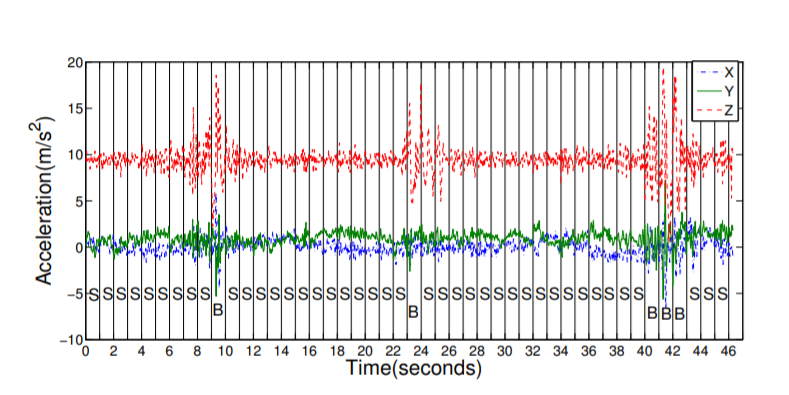
\includegraphics[width=0.75\textwidth]{Images/chapter2/relatedWork1.PNG}
 \caption{Accelerometer Data for three speedbreakers}
 \label{fig:graph}
  \end{figure}
  Et pour la détection du freinage du véhicule La technique utilisée est identique à celle de la détection des bosses,avec deux classes aussi étiquetées doux et freinage (smooth ‘S’, braking ‘R’) (Figure 2.2) :\newline
  \begin{figure}[h!]
    \center
    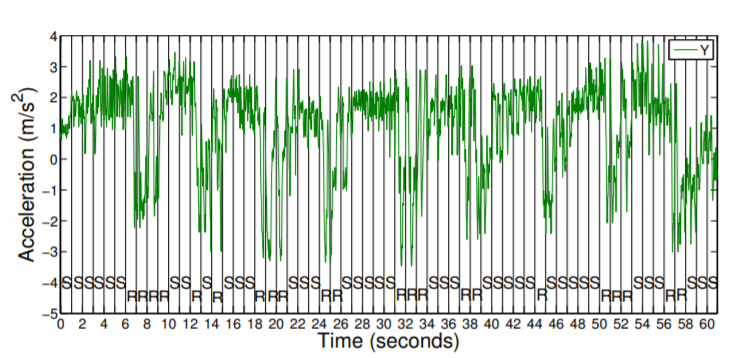
\includegraphics[width=0.75\textwidth]{Images/chapter2/relatedWork2.PNG}
   \caption{Braking events with generated class labels}
   \label{fig:graph}
    \end{figure}
    Ce  travail a été fait à Mumbai, L'algorithme identifie correctement 18 des 20 événements de bosse, Aucun tronçon de route lisse n'est identifié à tort comme une bosse. Ainsi, ils obtiennent un taux de faux négatifs de 10\% pour la détection des bosses et un taux de faux négatifs de 21,6\% et un taux de faux positifs de 2,7\% pour la détection de freinage.

  \subsection{Real time pothole detection using Android smartphones with accelerometer}
  Mednis et al., ont proposé un système de détection des nids-de-poule en temps réel basés sur des données d'accéléromètre pour le déploiement sur des appareils avec des ressources matérielles / logicielles limitées et leur évaluation sur des données du monde réel acquises à l'aide de différents téléphones intelligents basés sur Androïd OS. \newline
  ils ont utilisé un dispositif de collier LynxNet modifié \cite{PDFLynxNetWild} sur un route avec divers nids-de-poule pour la collecte des données des capteurs de l'accéléromètre.\newline 
  Après l'acquisition du premier data set de test, une recherche de fonctionnalités liées aux événements potentiels a été effectuée:\newline
  Le premier et le plus simple algorithme de détection d'événements ZTHRESH ont été testés sur l'ensemble de données acquis. Il est similaire à l'algorithme z-peak utilisé dans les systèmes Pothole Patrol \cite{PotholePatrolProceedings},Nericell\cite{mohanNericellUsingMobile2008}, et limite l'amplitude de l'accélération sur l'axe Z. Les caractéristiques qui classifient les mesures sont les valeurs dépassant des seuils spécifiques qui identifient le type des nids-de-pouls. \newline
  Pour la réorientation virtuelle, ils ont utilisé une approche plus simple: un placement contrôlé de l'accéléromètre, éliminant le traitement supplémentaire (Figure 2.3).\newline
  \begin{figure}[h!]
    \center
    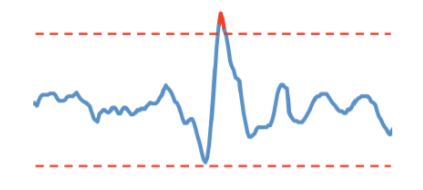
\includegraphics[width=0.75\textwidth]{Images/chapter2/relatedWork3.PNG}
   \caption{Pothole detection algorithm Z-THRESH. Events are represented by
   measurements with values exceeding specified threshold levels}
   \label{fig:graph}
    \end{figure}
    Ensuite, un algorithme légèrement plus avancé était le Z-DIFF (Figure 2.4) testé sur l'ensemble de données acquis. Contrairement à Z-THRESH, une recherche de deux mesures consécutives avec une différence entre les valeurs au-dessus du niveau de seuil spécifique a été effectuée. Ainsi, l'algorithme a détecté des changements rapides dans les données d'accélération verticale. L'algorithme nécessite la détermination de la position de l'axe Z de manière similaire à l'approche précédente. \newline
    \begin{figure}[h!]
      \center
      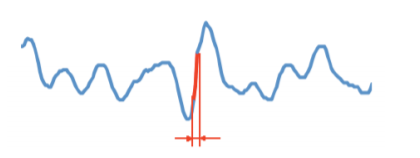
\includegraphics[width=0.75\textwidth]{Images/chapter2/relatedWork4.PNG}
     \caption{Pothole detection algorithm Z-DIFF. Events are represented by
     consecutive measurements with difference value above specific threshold level.}
     \label{fig:graph}
      \end{figure}
      les auteurs ont décidé de mettre en œuvre certaines des techniques utilisées pour le post-traitement. Une technique prometteuse pour la mise en œuvre sur un appareil à ressources limitées utilisait un écart type de l'accélération de l'axe vertical. Il a été implémenté dans l'algorithme STDEV (Z) (Figure 2.5) \newline

   \begin{figure}[h!]
      \center
      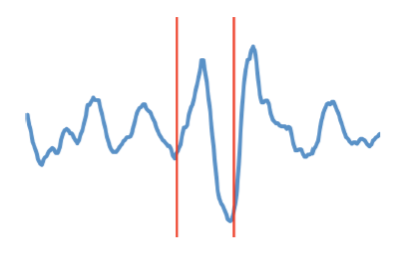
\includegraphics[width=0.75\textwidth]{Images/chapter2/relatedWork5.PNG}
     \caption{Pothole detection algorithm STDEV(Z). Events are represented by
     measurements with standard deviation value above specific threshold level.}
     \label{fig:graph}
      \end{figure}

      En utilisant des outils d'analyse visuelle de données et en recherchant des modèles de données spécifiques, les auteurs ont constaté qu'il existait certains événements caractérisés par un tuple de mesure spécifique. Toutes les données à trois axes de ce tuple avaient des valeurs proches de 0g. ils ont donc nommé cet algorithme G-ZERO (Figure 2.6).\newline


   \begin{figure}[h!]
      \center
      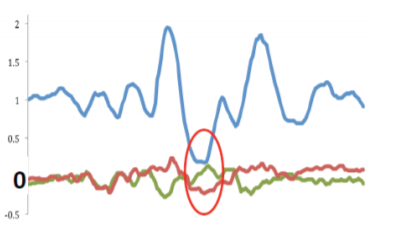
\includegraphics[width=0.75\textwidth]{Images/chapter2/relatedWork6.PNG}
     \caption{Pothole detection algorithm G-ZERO. Events are represented by tuple
     of measurements with all three axis values below specific threshold level.}
     \label{fig:graph}
      \end{figure}

      
les algorithmes ont détecté des irrégularités sur la route principale pour 100\% des grands nids-de-poule et 83 à 90\% des grappes de nids-de-poule; Selon l'algorithme, 78 à 89\% de la vérité terrain pour les petits nids-de-poule ont été détectés. Il est à noter que 9 d'entre eux (50\%) ont été détectés par les 4 algorithmes pour chacune des 10 sessions d'essai sur route
Et en gros, les tests d'évaluation ont abouti à une configuration optimale pour chaque algorithme sélectionné et l'analyse des performances dans le contexte de différentes classes d'irrégularité routière montre des taux de vrais positifs pouvant atteindre 90\%. \newline 



   Notre algorithme pour la détection de l'état de la route se distingue des travaux connexes de plusieurs côtés: \newline
Premièrement, nous ne détectons pas d'anomalies spécifiques, par contre nous concluons à l'état de la route en général. \newline
Deuxièmement, notre solution est plus simple en utilisant des ressources matérielles et logicielles limitées. \newline

\begin{table}[]
  \centering
  \resizebox{\textwidth}{!}{ %
  \begin{tabular}{lll}
    \hline
    Parameters & Wolverine & Mednis \\
    \hline
    Capteurs  & Accelerometre, Magnetometre, GPS  & Accelerometre, GPS \\
    \hline
Methodse pour la reorientation & Reorientation utilisant magnetometre et GPS bearing & Non défini \\
\hline
Valeur / Axes pris en compte & Z-axis Stdev sur une fenêtre de 1 sec du l'accéléromètre & Valeurs de l'axe Z de l'accéléromètre \\
\hline
Techniques utilisées & Machine Learning utilisé pour détecter les bosses et le freinage & Z-Thresh, ZDiff, STDEV, G-Zero \\
\hline
Taux d'échantillonnage réel de l'accéléromètre & 50 & 100 \\
\hline
Lieu d'expérimentation & IIT Bombay Campus & Vairoga iela, Riga, Latvia \\
\hline
Taux d'échantillonnage pris en compte par seconde & 50 values  & 100 values \\ 
\hline
Équipement utilisé pour la collecte de données & Capteurs de smartphone (Google Nexus S, HTC Wildfire S) & Samsung i5700 Samsung Galaxy S HTC Desire HTC HD2 \\
\hline
Véhicules utilisés & Suzuki Access 125, Autorickshaw & BMW 323 Touring (4-Wheeler) \\
\hline
Distance parcourue (km) / temps de trajet (heures) & Non reporté & 174 KM / Quelques semaines \\
\hline
Points de montage & Non défini (placé dans une certaine orientation arbitraire) & Tableau de bord avant \\
\hline
Objectif de la détection & Bosses, freinage & Nids de poule \\
\hline
Seuil 'threshold' utilisé & Non reporté & Z-Thresh = 0.4g Z-Diff = 0.2g STDEV = 0.2g G-Zero = 0.8g\\
\hline
Output & FN - 10\% (2 roues) FP - 8\% (3 roues) & 90\% des vrais positifs \\
\hline
Consommation d'énergie & Consomme 58\% moins d'énergie que Nericel & Non reporté \\
\hline
  \end{tabular} %
  }
  \caption{Inférences tirées Comparaison technique des travaux existants}
  \label{tab: my-table}
  \end{table}

  
  \section{L'acquisition des données}
  Notre système dépend de l'accéléromètre du smartphone attaché à un véhicule, produisant des résultats pour une condition de route donnée et sur la localisation précise de ces résultats à partir du GPS de ce smartphone.
Dans cette section, nous décrivons quelques expériences effectués par Pothole Patrol \cite{PDFPotholePatrol} pour valider le fonctionnement des capteurs d'un smartphone et la meilleure position où l'attacher.
\subsection{positionnement du smartphone}
Une préoccupation est que le placement du smartphone à l'intérieur du véhicule pourrait affecter la qualité du signal du capteur de l'accéléromètre. Pothole Patrol ont placé leurs accéléromètres à deux endroits à l'intérieur de la cabine d'une seule voiture. La (Figure 2.7) montre le signal de l'accéléromètre pour un tronçon fixe de chaussée à partir de deux positions de montage différentes: fixé au tableau de bord, et fixé sur le côté droit du pare-brise. Les signaux du tableau de bord et du pare-brise semblent assez similaires. \newline
  Par conséquent, ils ont fermement fixé l’accéléromètre au tableau de bord à l’intérieur de la boîte à gants de la voiture, qui est un endroit relativement facile pour installer des capteurs et qui les maintient hors de portée des passagers dans la cabine. Il en va de même pour les smartphones
  \begin{figure}[h!]
    \center
    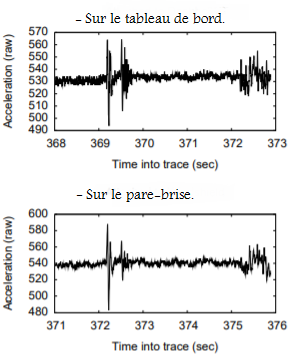
\includegraphics[width=0.75\textwidth]{Images/chapter2/positionmnt.PNG}
   \caption{Ces graphiques montrent comment le signal de l'accéléromètre (axe z) varie avec le placement à l'intérieur de la voiture selon Pothole Patrol.}
   \label{fig:smartphonePosition}
    \end{figure}


  \subsection{Méthode de récole de données}
  Pour la collecte de données, nous avons créé une application mobile qui utilise les capteurs du smartphone. Principalement l'accéléromètre et le GPS, ainsi que la vitesse de la véhicule et données d'autres capteurs tels que le capteur gyroscopique.\newline
  Tout cela sera discuté au chapitre N senction NN.

\section{Notre Approche}
Notre approche utilisera principalement le capteur d’accéléromètre comme entrées (input).
Ce Dernier signale l'accélération du véhicule le long des trois axes du capteur. \newline
 L'accélération mesurée comprend à la fois l'accélération physique du véhicule ainsi que celle de la gravité. La  mesure est signalée dans les champs Accel\_X, Accel\_Y et Accel\_Z. \newline
 En s’inspirant des travaux précédemment cités, considérer uniquement l’axe Z du capteur, en respectant le positionnement du téléphone donné, semble être une méthode à la fois simple et qui donne de bons résultats 

 Dans cette section, nous décrivons l'algorithme que nous avons développé pour détecter les conditions routières dans un enregistrement de données de capteur. \newline
Le problème de l'identification des conditions routières à partir des données de l'accéléromètre est difficile en raison de plusieurs facteurs tels que le comportement du conducteur (virages, dérapages, freinage brusque, conduite très basse, etc.) ou la grande variation et les conditions routières étranges ici en Algérie, donc notre algorithme suit 3 étapes principales:

\subsection{Windows split and Filtering}
  Cette étape est divisée en deux parties:
  \renewcommand{\labelitemi}{$\bullet$}
    \begin{itemize}
      \item \textbf{\textit{Windows split:}} Les données provenant de la partie d'enregistrement peuvent être pendant 1 mnt de conduite comme cela peut l'être pendant 1h de conduite, notre objectif principal de cette étude est de détecter l'état de la route à des distances spécifiques. L'algorithme proposé divise les données en plusieurs fenêtres en fonction de la distance et de l'heure de l'enregistrement.
      \item \textbf{\textit{Speed filtering:}} Une fois les données sont divisées en fenêtres; nous devons les filtrer avant le traitement, dans cette partie de filtrage de la vitesse (speed filtering) , les données dans lesquelles le véhicule ne se déplace pas ou se déplacent très lentement sont ignorées.
    \end{itemize}
    \textbf{ CAPTURE DE GRAPH}
\subsection{Smoothing and Threshold value}
  Une fois que l'algo a obtenu les données de filtrage, il commence à calculer la valeur moyenne de toutes les données afin d'identifier les anomalies de vibrations parmi les vibrations normales. \newline  
  Nous suivons deux méthodes pour calculer cette valeur moyenne chacune fournit un type différent de données de lissage, Nous notons que chaque méthode n'affecte pas les résultats finaux.
  
  \renewcommand{\labelitemi}{$\bullet$}
    \begin{itemize}
      \item \textbf{\textit{Average value of Waves smoothing:}} well tchika tchoka
      \item \textbf{\textit{Average value of Line smoothing:}} well tchoka tchika
    \end{itemize}
  Le moment où la valeur moyenne est détectée et en nous inspirant de nombreux articles de recherche dans ce domaine, nous avons choisi 0,8 g comme valeur sensible afin de calculer le seuil. \newline
  \textbf{AJOUTER LA FORMULE + CAPTURE DE GRAPH}


\subsection{Z-peak}
Après  que les données sont prêtes à être traitées; et que la valeur seuil est indiquée, on s'intéresse aux points de pics en dehors de cette valeur qui représentent les événements d'anomalie. \newline
Une fois cela fait, nous détectons si le niveau de la route est 0 (route lisse), 1 (route anormale) ou 2 (route très anormale) en divisant le nombre d'anomalies par la distance.